% !TeX root = ../dokumentation.tex
\setpagestylefoot
\renewcommand{\thefigure}{A\arabic{figure}}
\renewcommand\thelstlisting{A\arabic{lstlisting}}
\renewcommand\thetable{A\arabic{table}}
\newcommand*{\fullref}[1]{\hyperref[{#1}]{\ref*{#1}. \nameref*{#1}}} 

% Nummer des Inhaltes mit \setcounter{figure}{"`Number"'} (figure, lstlisting or table) ändern wenn nötig

\addchap{\langanhang}


% Quellenverzeichnis nach Literatur und Weblinks trennen
%\printbibliography[heading=subbibintoc,title={Literatur},nottype=online]
%\printbibliography[heading=subbibintoc,title={Weblinks},type=online]

% Quellenverzeichnis nicht trennen
\ifliteratur
    \printbibliography[heading=subbibintoc]
\fi

% Glossar
\ifglossar
    \printglossary[style=altlist,title=\langglossar]
\fi

\newpage
\addsec{Aufteilung der Kapitel}
\begin{table}[H]
	\centering
	\caption{Aufteilung der Kapitel}
	\begin{tabular}{|l|l|}
		\hline
		\textbf{Kapitel} & \textbf{Author} \\\hline
		\fullref{chap:einleitung} & Alexander Kehrer \\\hline
		\fullref{sec:photodioden} & Marcel Wagner \\\hline
		\fullref{sec:schrittmotoren} & Alexander Kehrer \\\hline
		\fullref{chap:grund_lidar} & Marcel Wagner \\\hline
		\fullref{chap:stand_der_technik} & Marcel Wagner\\\hline
		\fullref{chap:machbarkeitsstudie} & Marcel Wagner \\\hline
		%\fullref{chap:matlab_modell} & Alexander Kehrer \\\hline
		\fullref{chap:mechanik} & Marcel Wagner \\\hline
		\fullref{chap:hardware} & Alexander Kehrer \\\hline
		\fullref{chap:code} & Marcel Wagner \\\hline
		\fullref{chap:auswertung_matlab} & Alexander Kehrer \\\hline
		\fullref{chap:validierung} & Alexander Kehrer \\\hline
		\fullref{chap:fazit} & Alexander Kehrer \\\hline
		\fullref{chap:ausblick} & Marcel Wagner \\\hline
	\end{tabular}
\end{table}

\newpage
\addsec{Github Repository}
Im Rahmen der Studienarbeit wurde ein Github Repository zur Verwaltung der Daten angelegt. Da die Dateien sehr umfangreich sind, wird auf ein einzelnes Einfügen verzichtet und stattdessen ein Verweis auf das Repository eingebracht.\\
Github Repository: \href{https://github.com/WagnerMarcel/LIDAR}{https://github.com/WagnerMarcel/LIDAR}
\begin{table}[H]
	\centering
	\caption{Verweise auf Github Repository}
	\begin{tabular}{|l|l|}
		\hline
		\textbf{Kapitel} & \textbf{Anhang} \\\hline
		\fullref{chap:einleitung} & - \\\hline
		\fullref{chap:grundlagen_et} & - \\\hline
		\fullref{chap:grund_lidar} & - \\\hline
		\fullref{chap:stand_der_technik} & -\\\hline
		\fullref{chap:machbarkeitsstudie} & \href{https://github.com/WagnerMarcel/LIDAR/tree/master/04_Protokolle}{Protokolle zu den Versuchen} \\\hline
		%\fullref{chap:matlab_modell} & \href{https://github.com/WagnerMarcel/LIDAR/tree/master/06_Matlab\%20Modell}{Matalb code zum Modell} \\\hline
		\fullref{chap:mechanik} & \href{https://github.com/WagnerMarcel/LIDAR/tree/master/08_Mechanik}{Technische Zeichnungen} \\\hline
		\fullref{chap:hardware} & \href{https://github.com/WagnerMarcel/LIDAR/tree/master/05_Datenblätter/VL53L1X}{Datenblätter} \& \href{https://github.com/WagnerMarcel/LIDAR/tree/master/09_Platinen}{Platinen}\\\hline
		\fullref{chap:code} & \href{https://github.com/WagnerMarcel/LIDAR/tree/master/07_Code}{Code} \\\hline
		\fullref{chap:auswertung_matlab} & \href{https://github.com/WagnerMarcel/LIDAR/tree/master/11_Auswertung}{Matlab Code \& Bilder} \\\hline
		\fullref{chap:validierung} & - \\\hline
		\fullref{chap:fazit} & - \\\hline
		\fullref{chap:ausblick} & - \\\hline
	\end{tabular}
\end{table}

\newpage
\addsec{Technische Zeichnungen}
\begin{figure}[H]
	\centering
	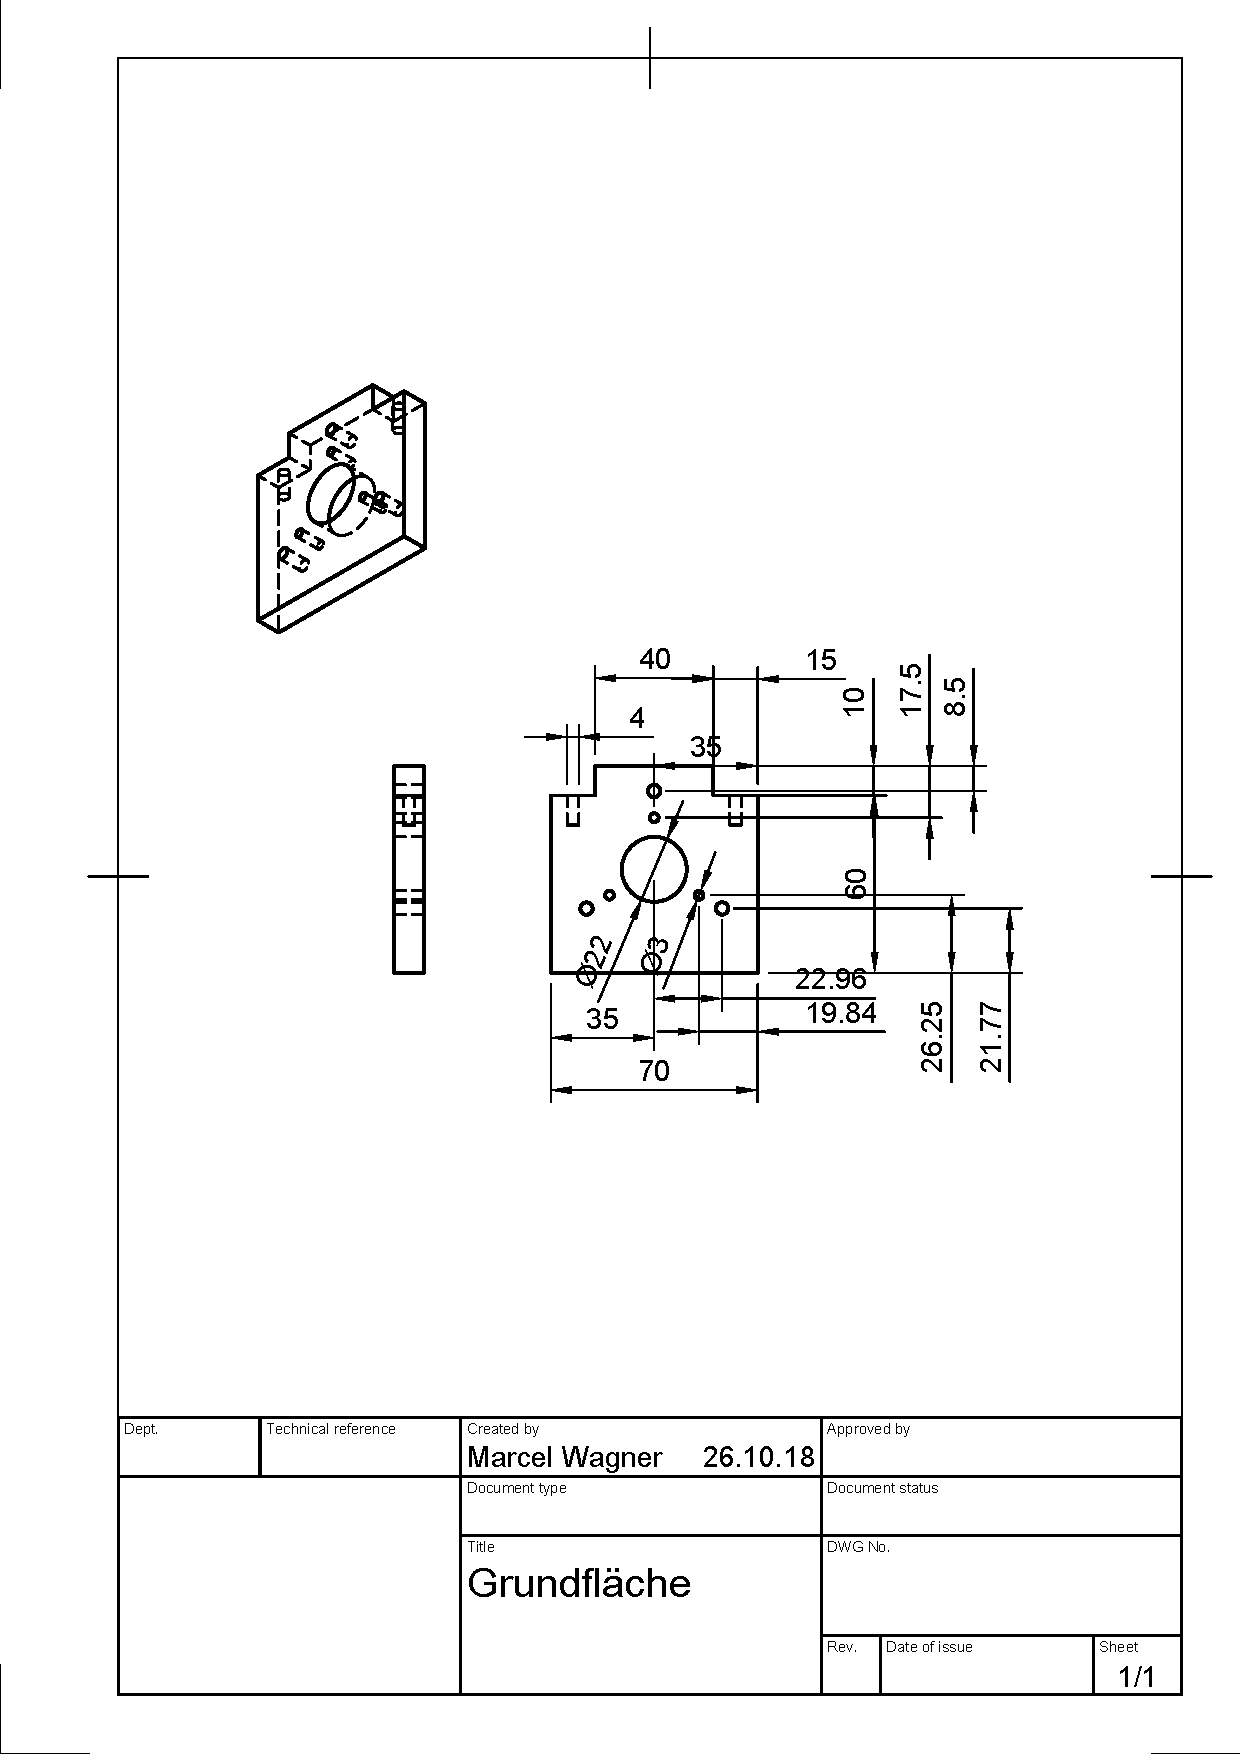
\includegraphics[width=0.95\textwidth]{images/Mechanik/Grundflaeche}
	\caption{Grundfläche}
\end{figure}
\begin{figure}
	\centering
	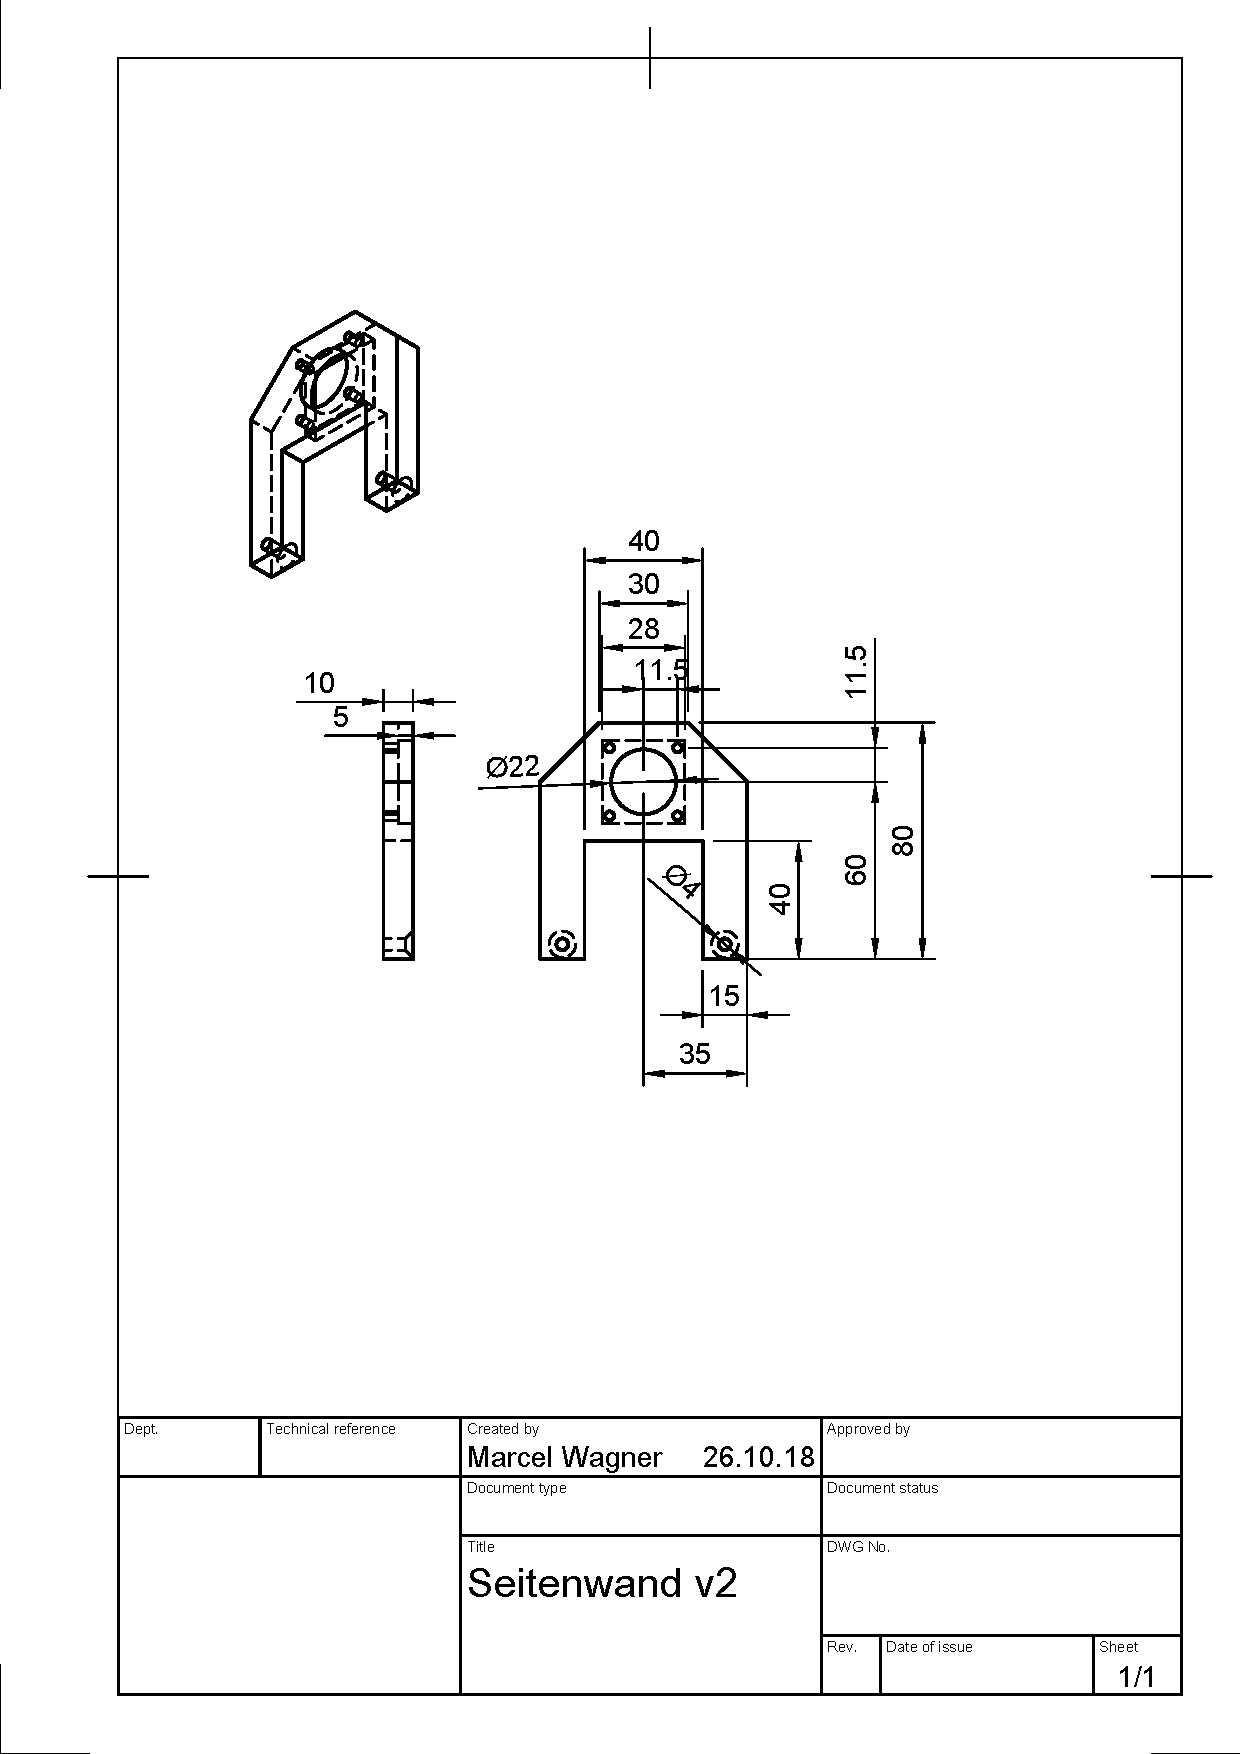
\includegraphics[width=\textwidth]{images/Mechanik/Seitenwand}
	\caption{Seitenwand}
\end{figure}

\begin{figure}
	\centering
	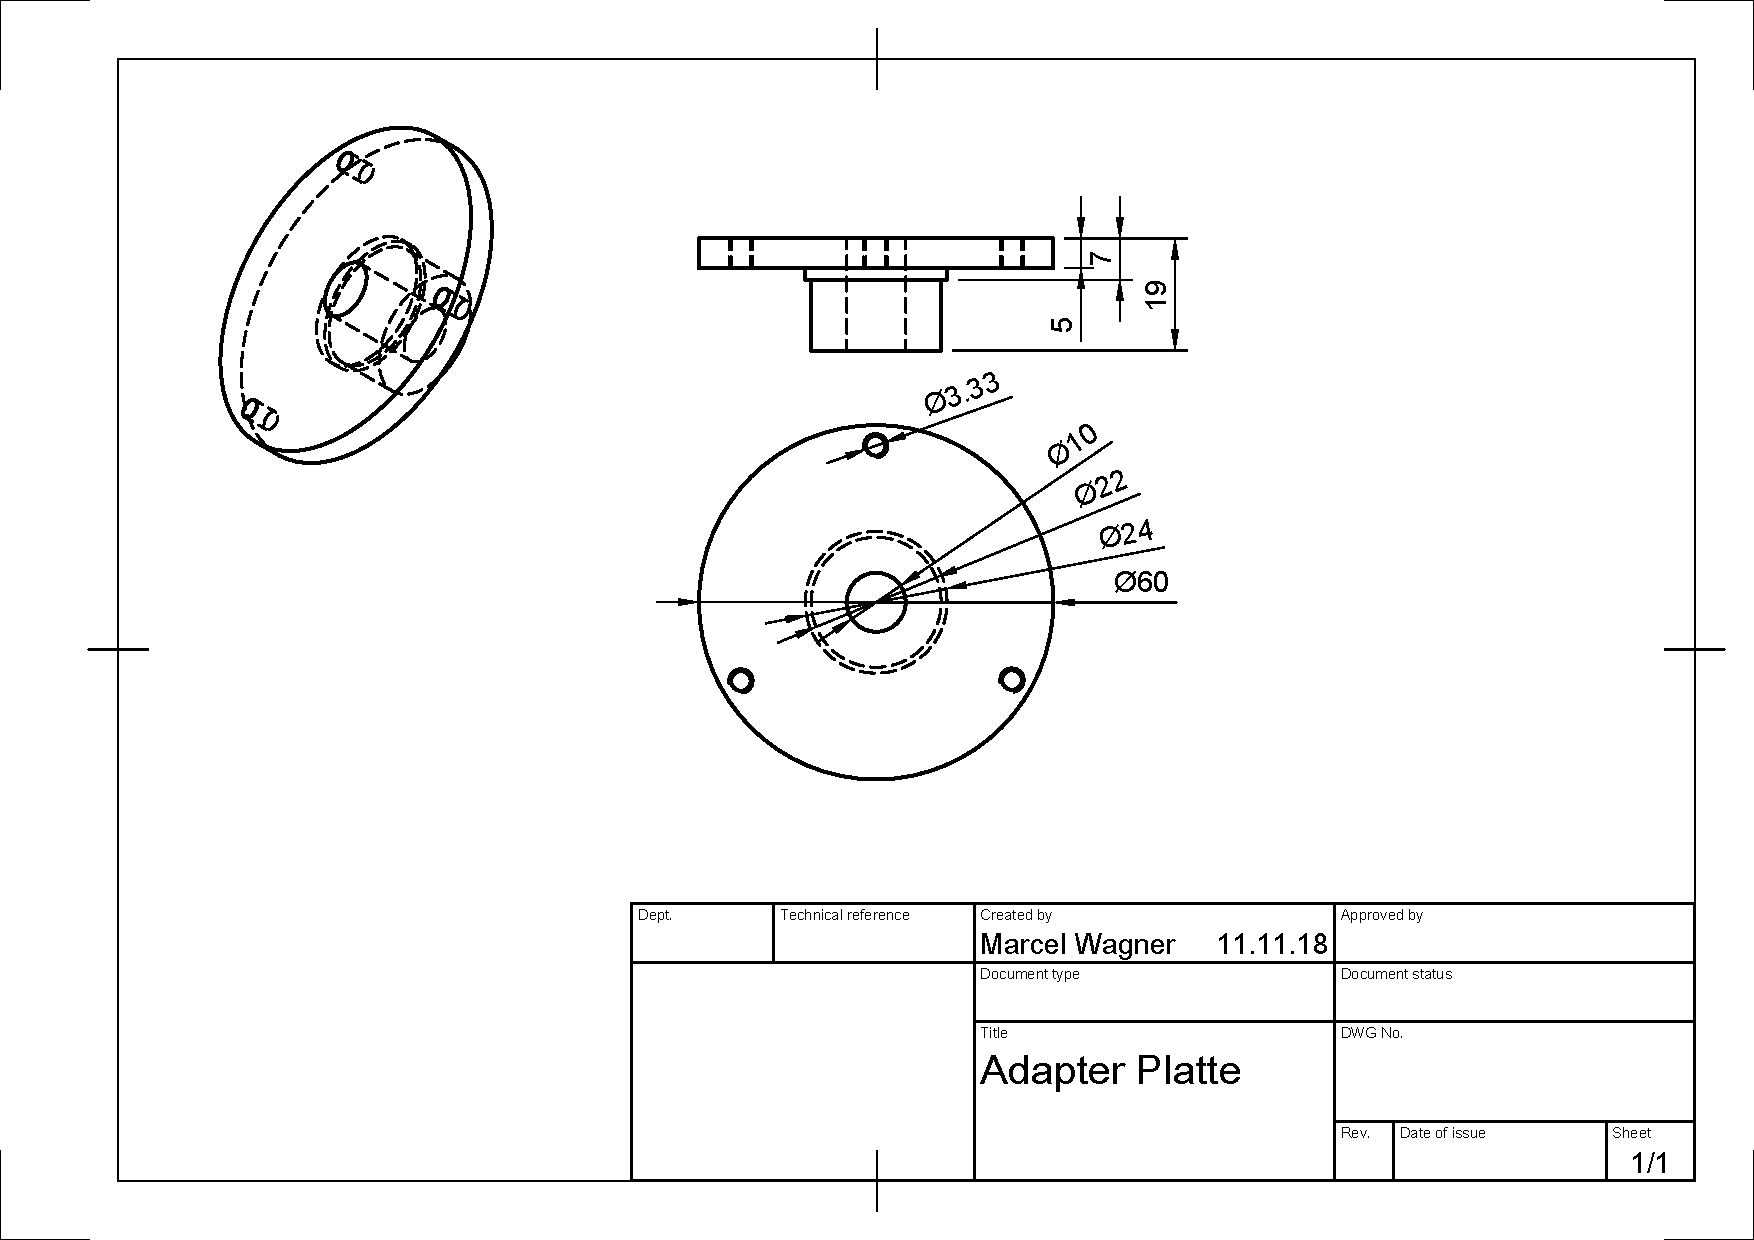
\includegraphics[angle=90,origin=c, width=\textwidth]{images/Mechanik/Adapterplatte}
	\caption{Adapterplatte}
\end{figure}
\begin{figure}
	\centering
	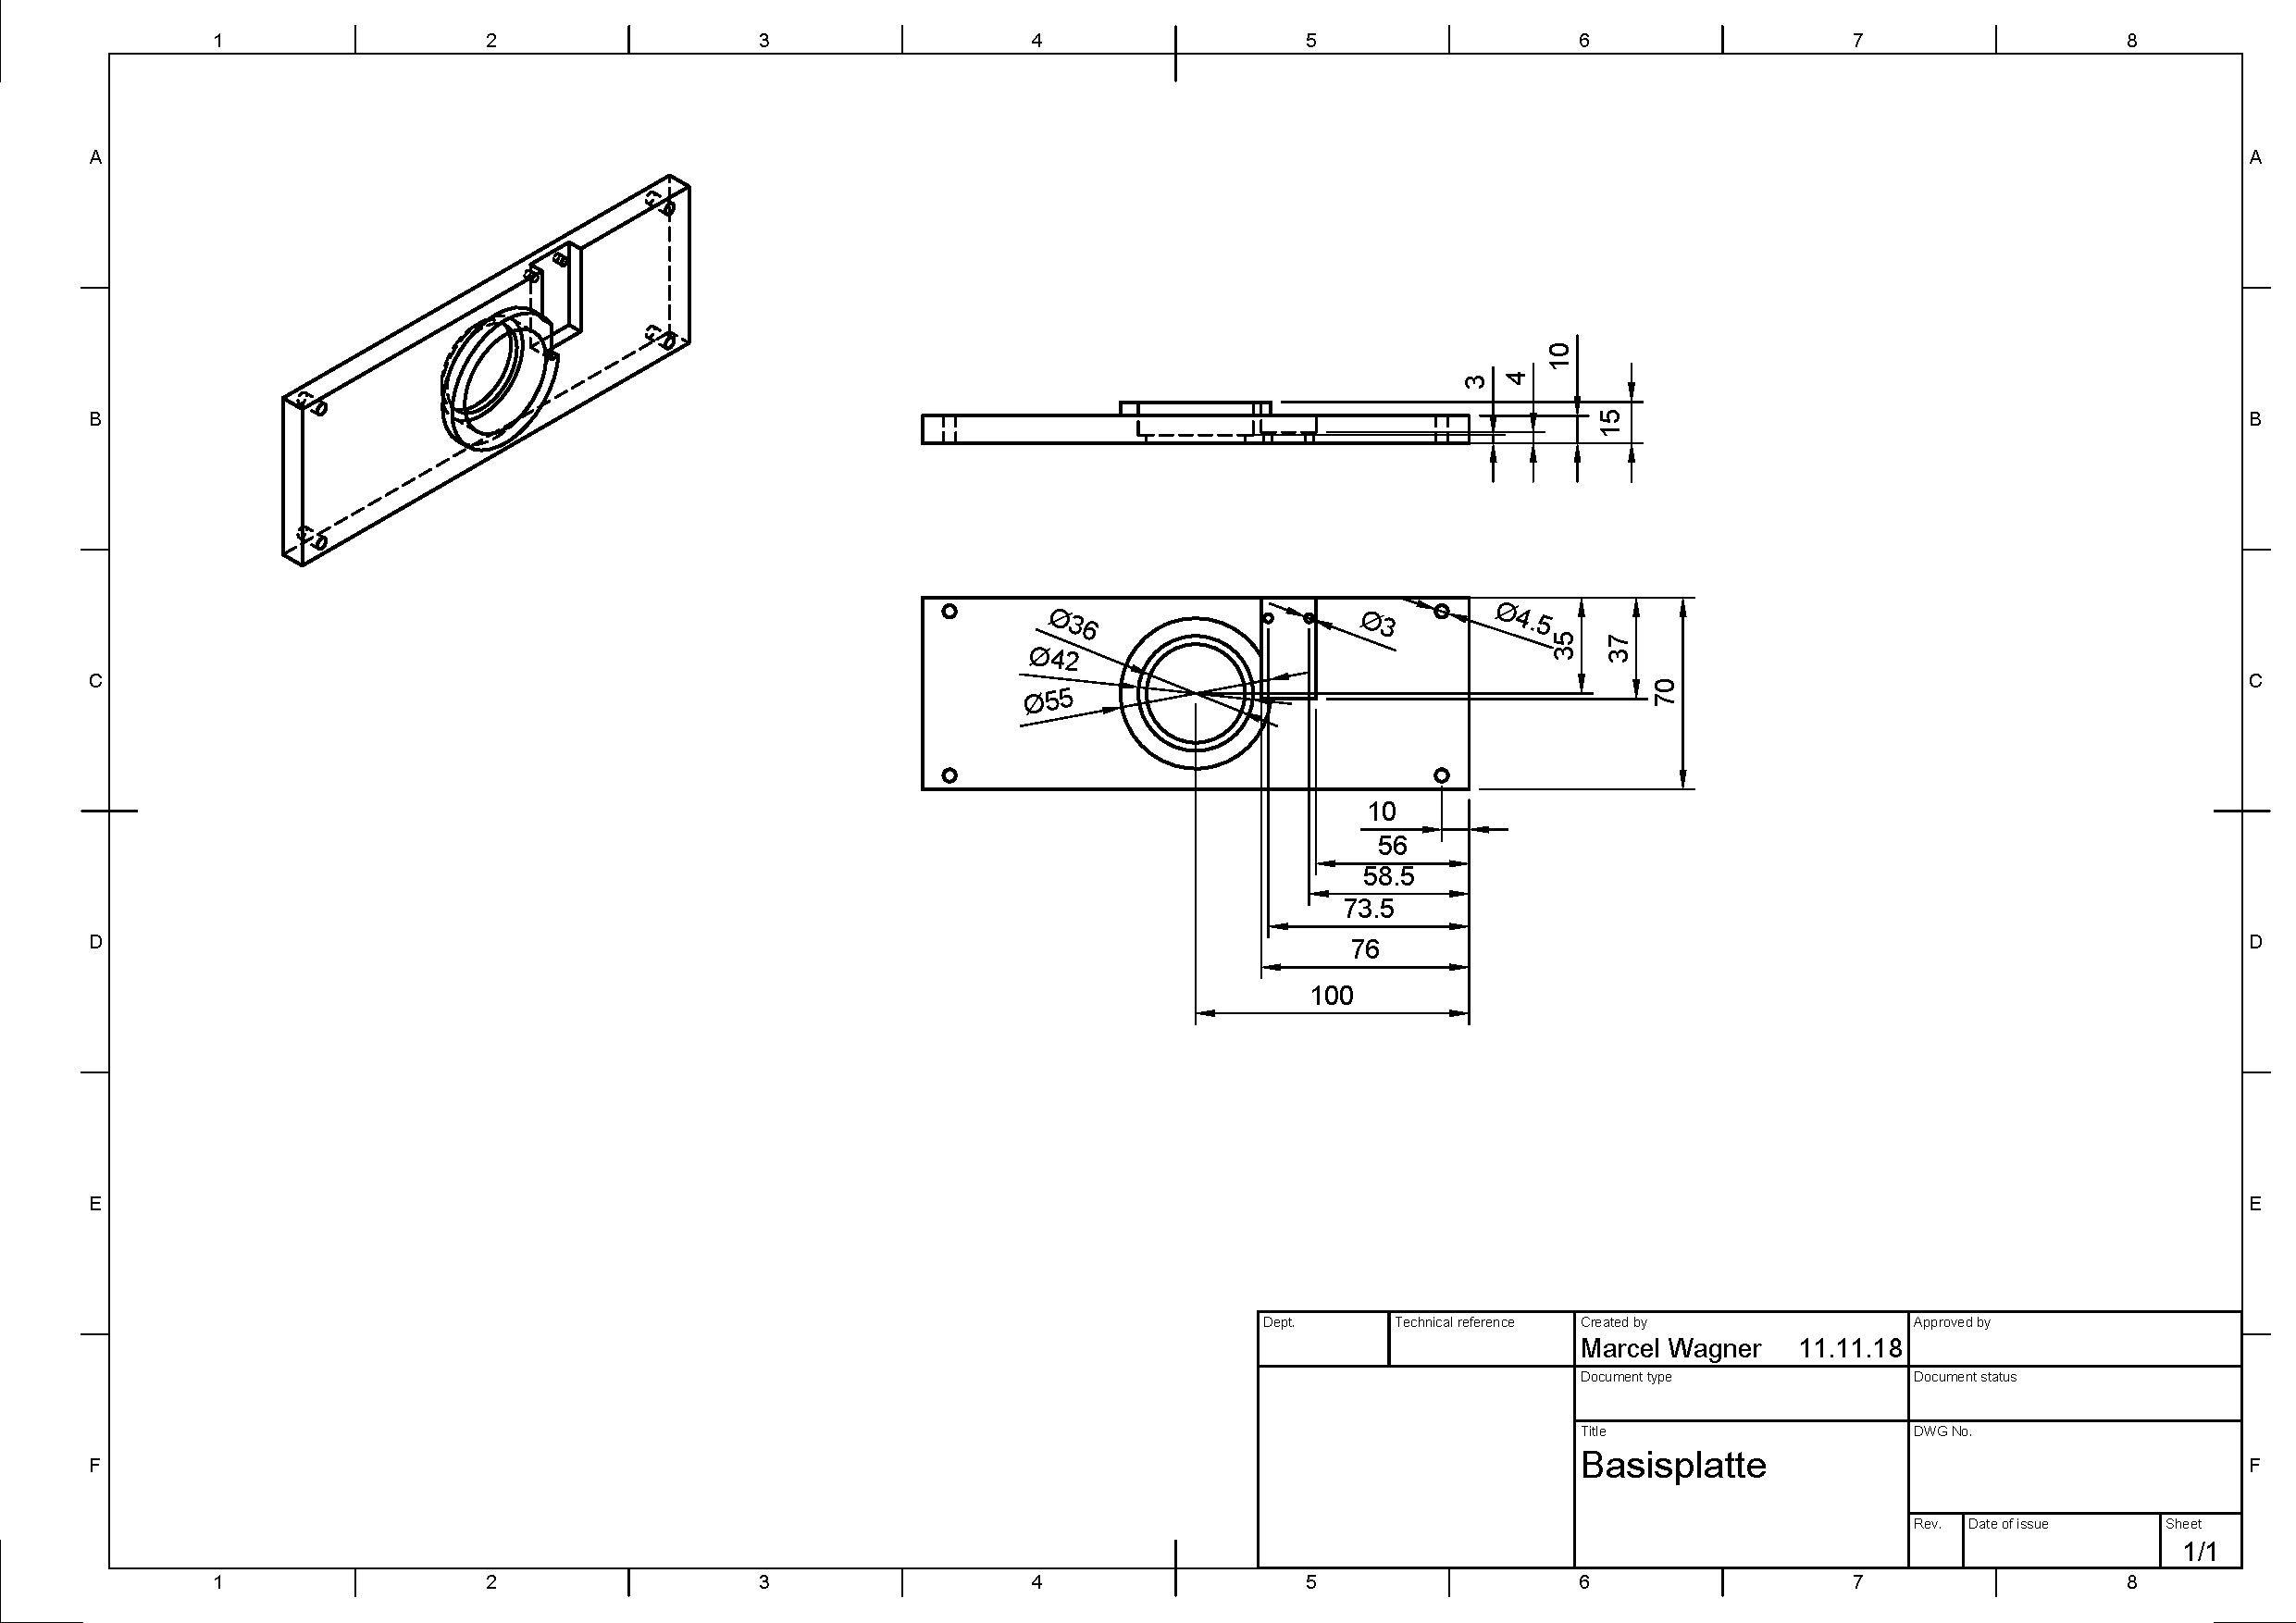
\includegraphics[angle=90,origin=c, width=\textwidth]{images/Mechanik/Basisplatte}
	\caption{Basisplatte}
\end{figure}



\begin{figure}
	\centering
	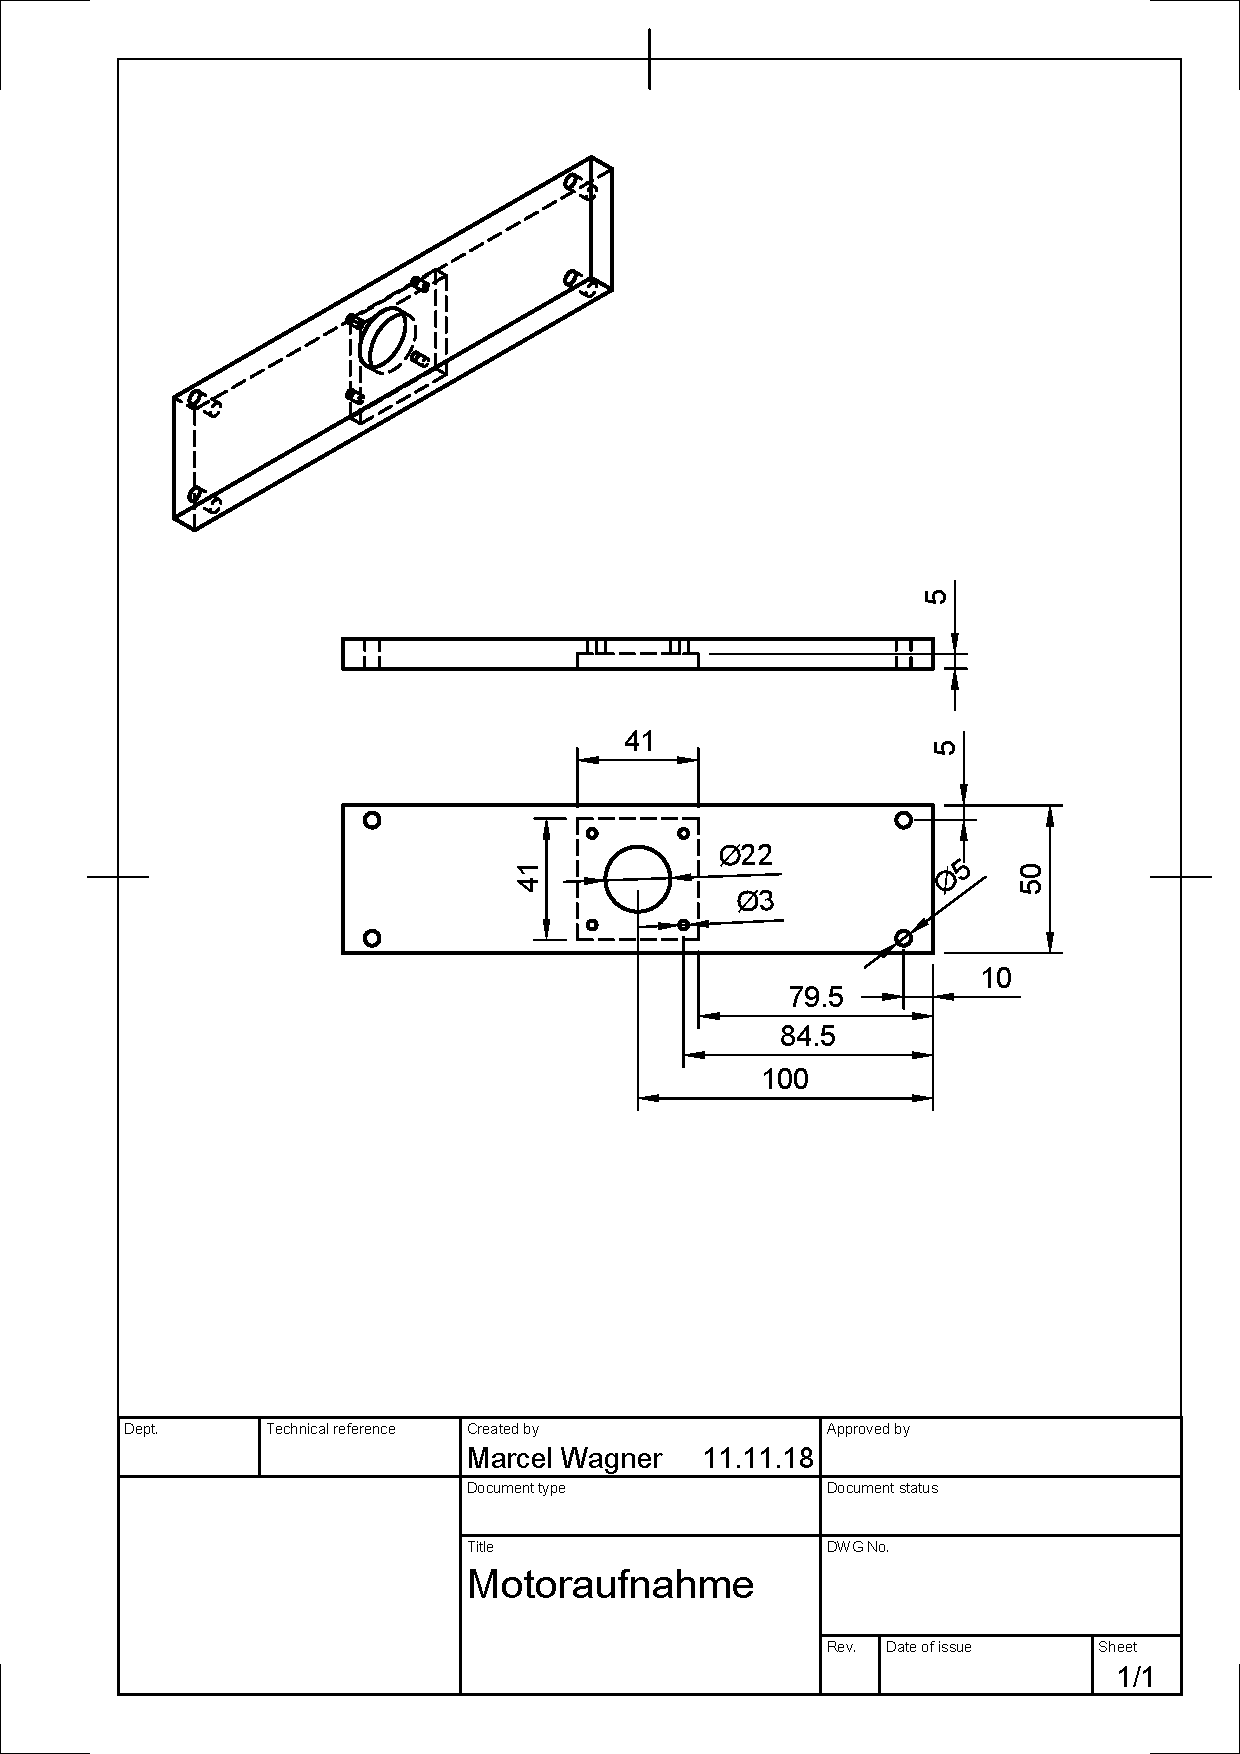
\includegraphics[width=\textwidth]{images/Mechanik/Motoraufnahme}
	\caption{Motoraufnahme}
\end{figure}
\begin{figure}
	\centering
	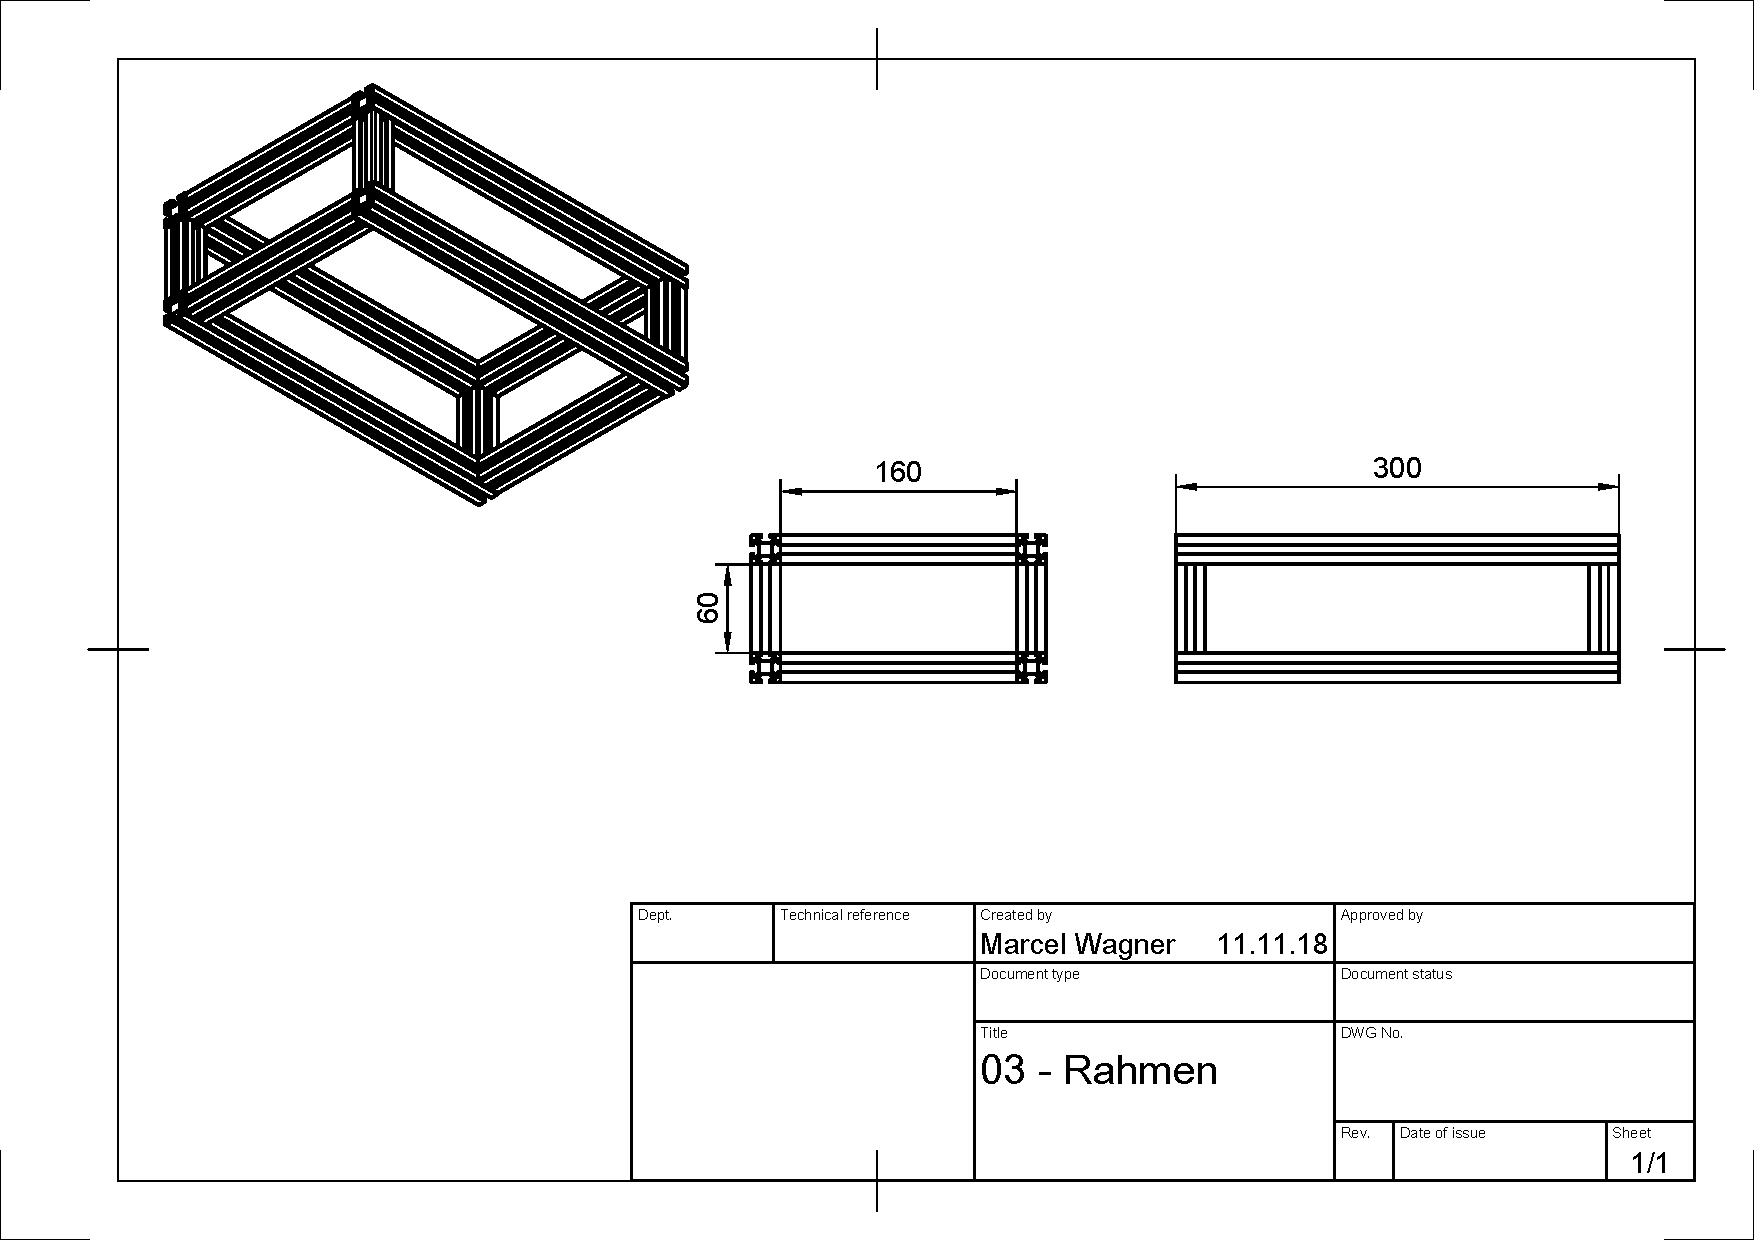
\includegraphics[angle=90,origin=c, width=\textwidth]{images/Mechanik/Rahmen}
	\caption{Rahmen}
\end{figure}


